\subsection{Репликация}

\begin{definition}
	\textit{Репликация} -- поддержание одинаковых данных на нескольких узлах.
\end{definition}

\subsubsection{Реализация репликации}

Репликация бывает \textbf{синхронной} (с использованием распределенных транзакций) и \textbf{асинхронной} (информация до реплик доходит с задержками). С другой стороны, различают
схемы репликации \textbf{c основной копией} и \textbf{симметричную}.

\paragraph{Репликация с основной копией}

\begin{figure}[h]
	\centering
	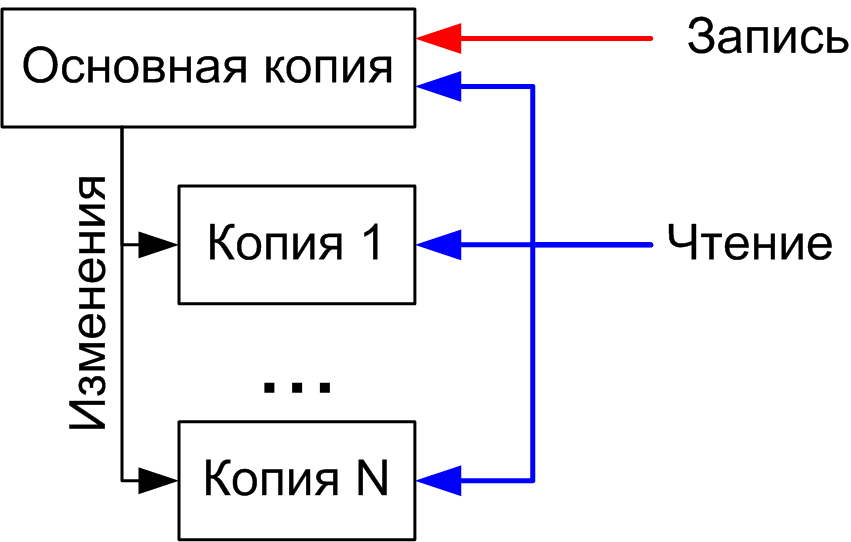
\includegraphics[width=0.8\textwidth]{../assets/kgeorgiy/distributed/Replication_Master.png}
	\caption{Схема репликации с основной копией}
	\label{repl-master}
\end{figure}

Чтение данных можно производить из любой копии БД, в то время как запись -- только в основную.
Согласованность всех копий обеспечивается за счет проверки при записи в основную копию. Данная
схема подходит, если число записей сильно меньше числа чтений.

\paragraph{Симметричная репликация}

\begin{figure}[h]
	\centering
	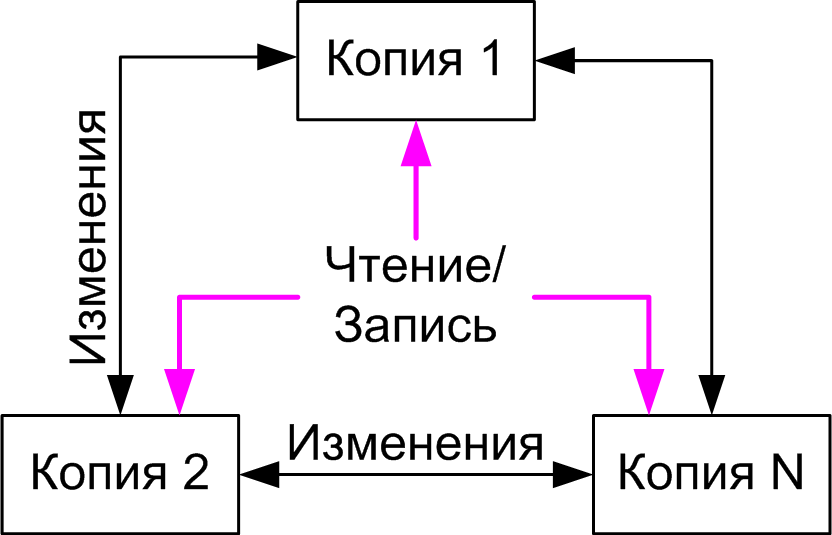
\includegraphics[width=0.8\textwidth]{../assets/kgeorgiy/distributed/Replication_Symmetric.png}
	\caption{Схема симметричной репликации}
	\label{repl-symm}
\end{figure}

Чтение и запись производятся в каждую копию независимо, все копии равноправны и автономны. Для
борьбы с противоречивыми изменениями в данной схеме требуется синхронность изменений.

\paragraph{Реализация репликации}

Данные об изменениях можно рассылать из журнала транзакций. Можно рассылать данный в различной
гранулярности:

\begin{itemize}
	\item \textbf{Репликация операторов}. При таком подходе используется меньше данных. Однако,
	      каждый оператор должен быть детерминированным, а также необходимо учитывать взаимный порядок
	      выполнения транзакций. Сложно для реализации.
	\item \textbf{Репликация записей}. Рассылается информация об изменении отдельных записей. При
	      таком подходе нет требования к детерминированности. Однако, крупные обновления данных приведут к
	      рассылке больших сообщений.
\end{itemize}

\subsubsection{Применения репликации}

\paragraph{Вертикальное масштабирование}

При необходимости вертикального масштабирования (наращивания мощности системы) следует использовать
\textbf{асимметричную схему}. Напомним, что ее использование целесообразно, когда количество изменений
гораздо меньше количества чтений.

Применяется в ситуациях, когда допустима асинхронность. Например, в Web-серверах и ERP-системах.

\paragraph{Горизонтальное масштабирование}

В ситуациях, когда необходимо производить множество локальных операций, например, в разных
географических областях, применяется \textbf{симметричная схема}. Каждая реплика отвечает за
определенные данные в зависимости от запроса. Также этот подход полезен в случае непостоянной
связи.

\paragraph{Повышение доступности}

Для повышения доступности данных следует использовать \textbf{асимметричную схему}, которая позволяет
менять основную реплику при выходе из строя прошлой. В случае синхронной репликации потери данных
отсутствуют, однако, в случае асинхронной вышедшая из строя основная реплика могла не успеть
разослать другим репликам изменения.

Также полезно \textbf{резервное копирование} БД. В асимметричной схеме для этого достаточно создать
реплику, с которой постоянно синхронизируется основная. Для создания резервной копии достаточно
отключить такую реплику, скопировать данные, включить обратно в систему и восполнить пропущенные
обновления.

\paragraph{Преобразование данных}

Используется \textbf{асимметричная схема}, которая предоставляет отлаженный способ получения всех
изменений данных. На основе них можно строить преобразование данных: изменение формата хранения,
консолидация, унификация, подсчет статистики и так далее. Таким образом, преобразования происходят
при репликации.